\chapter{Documentation}

\section{User documentation}
All of the pages are accessible from the homepage and/or the collapsable navbar in the top right.

\subsection{Registering and logging in}
While not logged in only graph view, about page and welcome page are accessible.

To register click on the register button on the homescreen.
The registration requires selecting a unique username, email and password.
The password has security requirements which are displayed immediately
after opening the form and in case of not meeting the criteria on submit.

To log in click on the login button on the homescreen. The login requires a username or email and password.

At this point the email is not used anywhere and is only included in preparation for email verification functionality.

\subsection{Opening a thought}
There are multiple ways to open a thought:
\begin{itemize}
  \item \textbf{New thoughts log on homepage} - On homepage there is a feed of the last three thoughts created on the website.
  Clicking on one of them will open the thought in graph view.
  
  Clicking on the "All Thoughts" button under the feed leads to all thoughts list.
  \item \textbf{Notifications} - The Notifications button and the bell icon in the navbar lead to the list of replies.
  Replies are thoughts of other users that linked to any of the logged-in user's thoughts.
  Clincking on a reply opens the respective thought.
  \item \textbf{Graph view} - The main way to access thoughts is through the graph view. We will take a closer look at it in the next section.
  \item \textbf{Direct link} - Every thought has a unique ID which can be shared and accessed directly using the URL in format '/graph/\{thoughtId\}'.

  Example of the full URI leading to the thought with ID 1: https://aphantasia.io/graph/1
\end{itemize}

\subsection{Graph view}
To access graph view either click the "Graph" button on the main page
or click on the graph icon in the navbar (three conected nodes).

In graph view you can use the following controls:
\begin{itemize}
  \item \textbf{Mouse wheel or bottom right buttons} - Zooms in and out

  Once zoomed past a threshold titles of the thoughts appear. (figure \ref{obr:afantazie_floating_titles})
  \item \textbf{Draging the background} - Pans the viewport
  \item \textbf{Dragging a node} - Moves the grabbed thought around
  
  This is useful for customizing the layout, "untying" thoughts that are too close to each other or to speed up the process of the layout algorithm. 
  \item \textbf{Clicking a node} - Highlights a thought and switches to highlighted mode.
\end{itemize}

\subsubsection*{Highlighted mode}

In default mode the whole display is used to view the graph and the user can interact with it as described above.
When a thought is accessed the graph view switches to highlighted mode. (figure \ref{obr:afantazie_mobile_graph_view})

In highlighted mode half of the screen gets dedicated to the highlighted thought preview and the other half to the graph view.

The graph view in highlighted mode shares almost all behavior with the default mode with a few exceptions:
\begin{itemize}
  \item \textbf{Visual node highlight} - The currently opened thought is also visually highlighted by a white circle around it.
  \item \textbf{Visual edges highlight} - All edges connected to the opened thought are exaggerated in thickness and color while all other egdes are dimmed.
  \item \textbf{Neighborhood thoughts} - On highlighting a thought the application loads its neighborhood.
\end{itemize}
Every time a thought is selected the viewport also smoothly centers on it.

The thought preview shows title, author, time of creation, content with clickable links and replies section.
Both the links in content and titles in replies section are color-coded based on authors selected color
and on click will highlight the respective thought.
At the bottom of the preview there are Reply button and a close button (up icon on mobile and X on desktop).

\subsubsection*{Neighborhood thoughts and graph walk}

When a thought is highlighted the application loads its neighborhood.
The neighborhood is defined as thoughts accessible through \gls{BFS} up to a given depth.
The currently used depth of the search is fixed at 3.

Some of the thoughts rendered on screen can be filled with black color. \ref{obr:afantazie_mobile_graph_view}
This indicates that some neighbors of the node are not visible on screen and thus the node is explorable.
  
\subsection{Creating a new thought}

There are two ways to access the thought creation page:
\begin{itemize}
  \item \textbf{From the graph view} - Click on the "New thought" button on the bottom of the graph view.
  \item \textbf{From the thought preview} - Click on the "Reply" button at the bottom of the thought preview.
\end{itemize}

Both of these ways lead to the thought creation page (figure \ref{obr:afantazie_thought_creation_page}).
The difference between them is that when accessed through the Reply button the respective thought link
is automatically added to the content input.

The thought creation page consists of two text fields: Title and Content.

Both the title and content are required. Title has a minimum length of 1 character. The content's minimum length is 5 characters.
Both of these requirements are enforced by validation rules and the user is notified by notification messages if the submit fails.

\subsubsection*{Referencing other thoughts}
When you add a link (or a reference) to a thought it will be connected and attracted the corresponding node in graph view.
Links can be added into the content field as a link with format "[id](text)"
where id is the id of the thought and text is the text that will be displayed.
The text does not have to necessarily be the original title of the linked thought.

Adding links can be done by three ways:
\begin{itemize}
  \item \textbf{Manually} - By typing the link in the content field
  \item \textbf{By 'Add reference' button} - This button opens a overlay with list of thought ttles and a search bar.
  Click on a thought title to add it at your cursor position.
  \item \textbf{Reply} - As mentioned, Reply button in graph view adds the link to the respective thought automatically.
\end{itemize}

Each thought can have up to five references.

\begin{figure}[p]\centering
  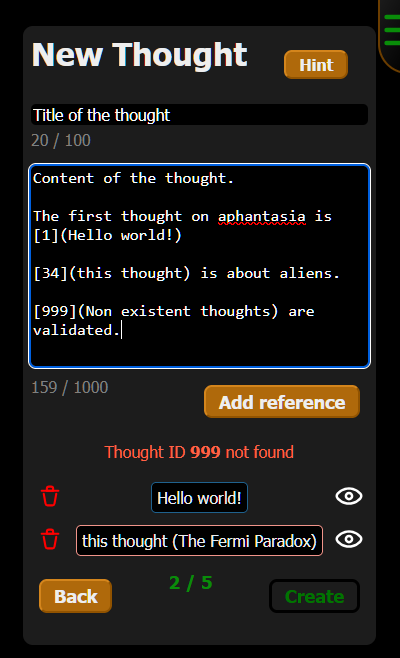
\includegraphics[width=80mm, keepaspectratio]{img/afantazie_thought_creation_page.png}
  \caption{Aphantasia - Thought creation page}
  \label{obr:afantazie_thought_creation_page}
\end{figure}

\subsection{Settings}
The settings page (figure \ref{obr:afantazie_user_settings}) is accessible from the navbar by clicking on the gear icon or by clicking the "User settings" button on the homepage.
Currently there are 2 settings that can be changed:
\begin{itemize}
  \item \textbf{On screen thought limit} - This setting changes the maximum number of thoughts that are be displayed on screen at once.
  The default value is 100. but can be changed to virtually any positive value.
  \item \textbf{Color} - This setting changes the color of users' thoughts in the graph view.
  There are predefined colors accessible by clicking the username but users are free to choose any color they like using a hexcode.
\end{itemize}

\begin{figure}[p]\centering
  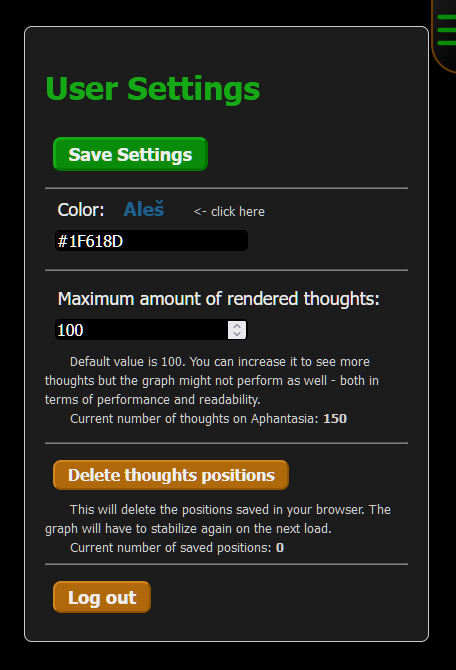
\includegraphics[width=80mm, keepaspectratio]{img/afantazie_user_settings.png}
  \caption{Aphantasia - User settings}
  \label{obr:afantazie_user_settings}
\end{figure}

Apart from these settings there is also a \textbf{Log out} button
and \textbf{Delete thought positions} button which erases positions of thoughts saved in the browser - forcing the graph to restabilize on next load.

\section{Developer documentation}
Here we will look at how to set up run the application locally. For more information about the architecture of the application, see chapter 4.

\subsection{Database}
Database is necessary for the application to run.
It is set up using Entity Framework Core and PostgreSQL but you can choose any other database engine supported by EF Core.
If you want to use a different engine, install the necessary packages
and replace the \textbf{UseNpsql} methods in these two files appropriately:
\begin{itemize}
  \item \textbf{Afantazie.Data.Model/DatabaseContextProvider.cs}
  \item \textbf{Afantazie.Data.Model/DesignTimeDataContextFactory.cs}
\end{itemize}

Once you have a database running you will have to scaffold the database (ie. create the schema compatible with Aphantasia).
To do so follow these steps:
\begin{enumerate}
  \item Add a file named \textbf{migrationsettings.json} in the root of project \textbf{Afantazie.Data.Model}.
  \item Add the following content to the file:
  \begin{lstlisting}
{
  "ConnectionStrings": {
    "DefaultConnection": "CONNECTION STRING TO YOUR DATABASE"
  }
}
  \end{lstlisting}
  \item Run the following command in the Data.Model project root:
  \begin{lstlisting}
    dotnet ef database update
  \end{lstlisting}
\end{enumerate}

The command should print the connection string you provided in the migrationsettings.json and ask for confirmation.
If everything is correct, confirm the prompt by inputting "y" and the database should be created.

\subsection{Frontend}
Before running the frontend make sure you have Node.js with npm installed on your machine.
Open the root of the AfantazieWeb directory in a command line and run:
\begin{lstlisting}
  npm install
  npm run dev
\end{lstlisting}

The application will then be accessible on the address seen in console output.
You can change the language of the application by changing \textbf{VITE\_LANGUAGE} to either 'en' or 'cz' inside the .env.development file.

\subsection{Backend}
Before running backend make sure you have .NET 8 SDK installed on your machine.

To run the Aphantasia backend we recommend using Visual studio and following these steps:
\begin{enumerate}
  \item Open the AfantazieServer.sln solution file in Visual Studio.
  \item Right click the AfantazieServer project and click on Manage User Secrets.
  \item Copy the json with connection string we provided in the database setup section and paste it into the secrets.json file.
  \item Set the AfantazieServer project as startup project and run it.
\end{enumerate}

You can configure the project in appsettings.Development.json file,
but it is not necessary for the application to run.

\subsection{Testing data}
Apart from adding testing data manually throught the appliaction or directly inserting into the database you can also use the Afantazie.Tools project.
It is a .NET 8 console application inside AfantazieServer solution
we created to help with varous tasks regarding Afantazie development.
Among other things it can generate random thoughts and users and add them to the database.

Before you run the tool to generate thoughts, follow these steps:
\begin{enumerate}
  \item Host and scaffold a database as described above.
  \item Manually remove foreign key constraints from the ThoughtReferences table.
  \footnote{This is necessary as the tool doesn't generate the data optimally and violates these constraints.
  You can add them back afterwards but it is not necessary for the application to run.}
  \item Create a appsettings.json in the root of the project.
  Its content should be the same as the migrationsettings.json shown above.
\end{enumerate}

Then set the project as startup project and run it.
Again the tool wil print the connection string and ask for confirmation after which you will be presented with several options.
There are a few random data generators but we recommend using option 3 - 'Generate random rainbow thoughts'.

This option will generate random clusters of thoughts where each generated thought has a set probability
of being linked to a thought in a different cluster.
You will then be asked for various parameters - fill them in and let the tool run.
Once it ends you will have a database filled with random clustered thoughts
and users with different colors across the color spectrum.